\documentclass[compress,aspectratio = 169]{beamer}
\usepackage{graphicx} % Required for inserting images
\usepackage{amsmath}

%\usepackage{mathspec}

\usetheme[progressbar=frametitle, numbering=none]{metropolis}
\useoutertheme[subsection=false]{miniframes}
%\useoutertheme{smoothtree}
\setbeamertemplate{section in toc}[sections numbered]
\useinnertheme{circles}

\usepackage{fontspec}

\defaultfontfeatures{Mapping=tex-text}
\setsansfont[Extension = .otf,
				BoldItalicFont=*-BoldItalic, 
             ItalicFont=*-RegularItalic, 
             BoldFont=*-Bold, 
             UprightFont=*-Regular]{SF-Pro-Text}
%\setmathfont(Digits,Latin,Greek){AvenirNext-Regular.otf}

\usecolortheme{ateneo}


\usepackage{booktabs}

\usepackage{upgreek}

\usepackage{xspace}
\newcommand{\themename}{\textbf{\textsc{metropolis}}\xspace}

\usefonttheme{professionalfonts}
\usepackage{unicode-math}

\title[Stock price prediction]{Using Transformer Model for stock price prediction}
\subtitle{Undergraduate thesis proposal presentation}
\author[Alejo, Nery, Realda]{Albert Matthew Alejo \and Jaime Angelo Nery \and Zielle Frances Realda}
\date{\today}
\institute[ADMU]{Ateneo de Manila University}

\usepackage{physics}

\setbeamertemplate{footline}
{
    \leavevmode%
    \hbox{%
        \begin{beamercolorbox}[wd=.33\paperwidth,ht=3ex,dp=1ex,center]{author in head/foot}%
            \usebeamerfont{author in head/foot}\insertshortauthor
        \end{beamercolorbox}%
        \begin{beamercolorbox}[wd=.34\paperwidth,ht=3ex,dp=1ex,center]{title in head/foot}%
            \usebeamerfont{title in head/foot}\insertshorttitle
        \end{beamercolorbox}%
        \begin{beamercolorbox}[wd=.33\paperwidth,ht=3ex,dp=1ex,right]{date in head/foot}%
            \usebeamerfont{date in head/foot}\insertshortdate{}\hspace*{2em}
            \insertframenumber{} / \inserttotalframenumber\hspace*{2ex} 
        \end{beamercolorbox}}%
        \vskip0pt%
    }
    \makeatother

\metroset{block=fill} 



\begin{document}

\maketitle

\begin{frame}{Outline}
\tableofcontents[hideallsubsections]
\end{frame}

\section[Introduction]{Projectile motion in two dimensions}

\subsection{Ideal model of projectile motion}

\begin{frame}{\subsecname}


The ideal model of projectile motion assumes that 

\begin{enumerate}
\item the acceleration due to gravity is constant and is pointing downwards and 
\item there is no air resistance.
\end{enumerate}

\end{frame}

\begin{frame}{\subsecname}

Let \(\mathbf{v}(0) \equiv \mathbf{v}_0\) be the initial velocity of an object pointed at an angle \(\theta\). According to Galileo, the horizontal and the vertical motion of the object is independent and can be expressed as the sum of both motions
 
\begin{equation}\mathbf{v}_0 = v_{0x}\hat{\mathbf{i}} + v_{0y}\hat{\mathbf{j}}\end{equation}

where

\begin{align}
&v_{0x} = |\mathbf{v}_0| \cos \theta, \\ 
&v_{0y} = |\mathbf{v}_0| \sin \theta.
\end{align}
\end{frame}

\begin{frame}{\subsecname}

Since the acceleration due to gravity is constant and only applies to the vertical direction, the velocity in the horizontal direction remains constant. The components of acceleration are:

\begin{align}
& a_x = 0, \\ 
& a_y = -g
\end{align}

where \(g\) is the acceleration due to gravity.

\end{frame}

\section{Concepts}

\subsection{Kepler's laws of planetary motion and the Kepler problem}

\begin{frame}{\subsecname}

Johannes Kepler first formulated the laws that describe planetary motion:

\begin{enumerate}

\item Each planet moves in an ellipse with the sun at one focus.\footnotemark

\item The sector from the sun to a planet sweeps out equal area in equal time.

\item The period of revolution \(T\) of a planet about the sun is related to the semi-major axis \(a\) of the ellipse by \(T^2 = ka^3\) where \(k\) is the same for all planets.
\end{enumerate}

\footnotetext{We will only be able to show this.}

\end{frame}

\subsection{Newton's law of gravitation}

\begin{frame}{\subsecname}
The gravitational force between two objects is directly proportional to the product of their masses and inversely proportional to the square of the distance between them, i.e.

\begin{equation}
F = G\frac{m_1m_2}{r^2}
\end{equation}

where \(m_1, m_2\) are the masses of two objects, \(r\) is the distance between the two objects, and \(G = 6.6743 \times 10^{-11} \text{m}^3 \cdot \text{kg}^{-1} \cdot \text{s}^{-2}\) is the gravitational constant.

\end{frame}

\section[Celestial mechanics]{Two-dimensional motion in celestial mechanics}


\subsection{Two-body problem}

\begin{frame}{\subsecname}

\begin{figure}
    \centering
    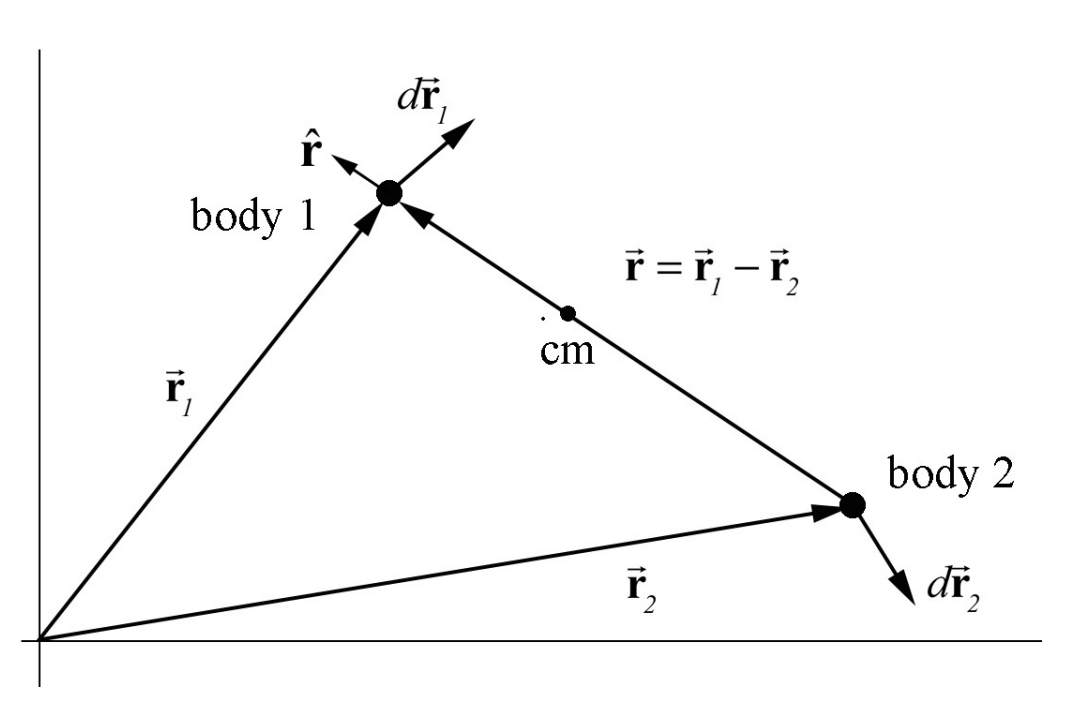
\includegraphics[height = 0.8\textheight]{assets/twobody.png}
    \caption{Coordinate system for the two-body problem.}
    \label{fig:my_label}
\end{figure}
\end{frame}

\begin{frame}{\subsecname}

% insert photo

System of two bodies and their gravitational effect toward each other:

\begin{equation}
\mathbf{F}_{12} = - \mathbf{F}_{21} \label{3rdlaw}
\end{equation}

in accordance with Newton's third law of motion.

\end{frame}

\begin{frame}{\subsecname}

\begin{block}{Two-body problem}

Let \(\mathbf{r}_1\) and \(\mathbf{r}_2\) be the position of bodies 1 and 2. The motion of the bodies is modeled by the equations

\begin{align}
\mathbf{F}_{12} = m_1\mathbf{r}''_1 \label{F1} \\ 
\mathbf{F}_{21} = m_2\mathbf{r}''_2 \label{F2}
\end{align}

\end{block}

\end{frame}


\subsection{Reducing the two-body problem into a one-body problem}

\begin{frame}{\subsecname}

The motion of two interacting bodies is equivalent to the motion of a single body acted on by an external central gravitational force where the mass of the single body is 

\begin{equation}
\frac{1}{\mu}= \frac{1}{m_1} + \frac{1}{m_2} \implies \mu = \frac{m_1m_2}{m_1+m_2}\footnotemark.
\end{equation}

\footnotetext{This central mass is located in between the two bodies, and the ratio of the distance between the a body and the central mass is equal to the inverse ratio of their masses.}

\end{frame}


\begin{frame}{\subsecname}

The force on body 1 can be described by

\begin{equation}
\mathbf{F}_{21} = -F_{21}\frac{\mathbf{r}}{r} =  -F_{21}\hat{\mathbf{r}} = -G\frac{m_1m_2}{r^2} \hat{\mathbf{r}}
\end{equation}

where \(F_{21} = |\mathbf{F}_{21}|\), \(r = |\mathbf{r}|\), and \(\hat{\mathbf{r}} = \frac{\mathbf{r}}{r}\).

\end{frame}

\begin{frame}{\subsecname}

Dividing through by the mass in both Equations \ref{F1} and \ref{F2},

\begin{align}
\frac{\mathbf{F}_{12}}{m_1} = \mathbf{r}''_1 \label{F1_1}\\ 
\frac{\mathbf{F}_{21}}{m_2} = \mathbf{r}''_2 \label{F2_1} 
\end{align}

\end{frame}

\begin{frame}{\subsecname}

Subtracting Equation \ref{F2_1} from Equation \ref{F1_1}, we get

\begin{equation}
\frac{\mathbf{F}_{12}}{m_1} - \frac{\mathbf{F}_{21}}{m_2} = \mathbf{r}''_1 - \mathbf{r}''_2 = \mathbf{r}''.
\end{equation}

Using the initial result on Equation \ref{3rdlaw}, we get

\begin{equation}
\frac{\mathbf{F}_{12}}{m_1} - \frac{-\mathbf{F}_{12}}{m_2} = \mathbf{F}_{12}\left(\frac{1}{m_1} + \frac{1}{m_2} \right) = \mathbf{F}_{12} \frac{1}{\mu} = \mathbf{r}''.
\end{equation}

\end{frame}

\begin{frame}{\subsecname}
And so, we reduce the system of two equations to

\begin{equation}
\mathbf{F}_{12} = \mu\mathbf{r}''.
\end{equation}

\end{frame}

\section{The orbit equation}

\subsection{Deriving the orbit equation}
\begin{frame}{\subsecname}

The (gravitational) potential energy with the choice of zero reference point \(U(\infty) = 0\) is 

\begin{equation}
U(r) = - \frac{Gm_1m_2}{r^2} r =- \frac{Gm_1m_2}{r}
\end{equation}

The total energy of the system is constant, so

\begin{equation}
E = \text{KE} + \text{PE} = \frac{1}{2}\mu v^2 - \frac{Gm_1m_2}{r} \label{E}
\end{equation}

where \(v\) is the scalar of the relative speed of two bodies -- i.e. \(v = |\mathbf{v}|\).
\end{frame}

\begin{frame}{\subsecname}
Choose polar coordinates such as 
\begin{align}
\mathbf{v} = v_r \hat{\mathbf{r}} + v_\theta \hat{\boldsymbol{\uptheta}} &&
v = |\mathbf{v}| = \sqrt{\left(\dv{r}{t}\right)^2 + \left(r\dv{\theta}{t}\right)^2}
\end{align}

where \(v_r = r'\) and \(v_\theta = \theta'\).

Equation \ref{E} becomes

\begin{equation}
E = \frac{1}{2} \mu \left[ (r')^2 + (r\theta')^2 \right] - \frac{Gm_1m_2}{r^2} \label{E2}
\end{equation}

\end{frame}

\begin{frame}{\subsecname}
The angular momentum with respect to the origin is 

\begin{equation}
\mathbf{L}_O = \mathbf{r}_O \times \mu\mathbf{v}= r\hat{\mathbf{r}} \times \mu(v_r\hat{\mathbf{r}} + v_\theta\hat{\boldsymbol{\uptheta}}) = \mu rv_\theta \hat{\mathbf{k}} = \mu r \theta' \hat{\mathbf{k}} =: L\hat{\mathbf{k}}
\end{equation}

where \(L = \mu rv_\theta = \mu r \theta'\)\footnotemark.

\footnotetext{\(L\) denotes the angular momentum of the body.}
\end{frame}

\begin{frame}{\subsecname}

We then remove the \(\theta\) dependence from Equation \ref{E2} using the result:

\begin{equation}
\theta' = \frac{L}{\mu r^2}
\end{equation}

We get

\begin{equation}
E = \frac{1}{2}\mu (r')^2 + \frac{1}{2} \frac{L^2}{\mu r^2} - \frac{Gm_1m_2}{r^2} \label{E3}
\end{equation}

\end{frame}

\subsection{Differential equation}

\begin{frame}{\subsecname}
We can rearrange Equation \ref{E3} to get a first-order differential equation:

\begin{block}{The orbit equation}
\begin{equation}
r' = \sqrt{\frac{2}{\mu}}\left( E - \frac{1}{2}\frac{L^2}{\mu r^2} + \frac{Gm_1m_2}{r^2} \right)^{\frac{1}{2}}
\end{equation}
\end{block}

\end{frame}

\begin{frame}{\subsecname}

Instead of solving \(r\) w.r.t. \(t\), we shall find a geometric description of the orbit by finding \(r(\theta)\):

\begin{align}
\dv{\theta}{r} = \frac{\theta'}{r'} &= \frac{L}{\mu r^2} \left[\sqrt{\frac{2}{\mu}}\left( E - \frac{1}{2}\frac{L^2}{\mu r^2} + \frac{Gm_1m_2}{r^2} \right)^{\frac{1}{2}}\right]^{-1} \\
&= \frac{L}{\sqrt{2\mu}} \frac{\dfrac{1}{r^2}}{\left( E - \dfrac{1}{2}\dfrac{L^2}{\mu r^2} + \dfrac{Gm_1m_2}{r^2} \right)^{\frac{1}{2}}} \label{diff}
\end{align}

\end{frame}

\begin{frame}{\subsecname}

We solve the differential equation in \eqref{diff}:

\begin{align}
\dv{\theta}{r} &= \frac{L}{\sqrt{2\mu}} \frac{\dfrac{1}{r^2}}{\left( E - \dfrac{1}{2}\dfrac{L}{\mu r^2} + \dfrac{Gm_1m_2}{r^2} \right)^{\frac{1}{2}}},\\
\dd \theta &= \frac{L}{\sqrt{2\mu}} \frac{\dfrac{1}{r^2}}{\left( E - \dfrac{1}{2}\dfrac{L}{\mu r^2} + \dfrac{Gm_1m_2}{r^2} \right)^{\frac{1}{2}}} \dd r.
\end{align}

\end{frame}

\begin{frame}{\subsecname}
We substitute \(u = \frac{1}{r}\) and \(\dd u = - \frac{1}{r^2}\dd r\) to get

\begin{align}
\dd \theta = -\frac{L}{\sqrt{2\mu}} \frac{\dd u}{\left( E - \dfrac{L^2}{2\mu}u^2 + Gm_1m_2u \right)^{\frac{1}{2}}},\\
\dd \theta = - \frac{\dd u}{\left[ \dfrac{2\mu E}{L^2} - u^2 +2 \left( \mu\dfrac{Gm_1m_2}{L^2}\right)u \right]^{\frac{1}{2}}}.
\end{align}
\end{frame}

\begin{frame}{\subsecname}
We define \(r_0 := \frac{L^2}{\mu Gm_1m_2}\footnotemark \)which simplifies our differential equation to

\begin{equation}
\dd \theta = - \frac{\dd u}{\left[ \dfrac{2\mu E}{L^2} - u^2 +\dfrac{2u}{r_0} \right]^{\frac{1}{2}}}
\end{equation}

\footnotetext{\(r_0\) is called the \textit{semilatus rectum}}

\end{frame}

\begin{frame}{\subsecname}
We now rewrite the denominator in order to express eccentricity.

\begin{align}
\dd \theta &= - \frac{\dd u}{\left[ \frac{2\mu E}{L^2} + \frac{1}{r_0^2} - u^2 +\frac{2u}{r_0} - \frac{1}{r_0^2} \right]^{\frac{1}{2}}}\\
&= -\frac{\dd u}{\left[ \frac{2\mu E}{L^2} + \frac{1}{r_0^2} - \left(u - \frac{1}{r_0}\right)^2\right]^{\frac{1}{2}}}\\
&= -\frac{r_0 \dd u}{\left[ \frac{2\mu E r_0^2}{L^2} + 1 - \left(r_0u-1\right)^2\right]^{\frac{1}{2}}}
\end{align}

\end{frame}

\begin{frame}{\subsecname}
We define \(\varepsilon^2 := \frac{2\mu Er_0^2}{L^2} + 1 \footnotemark\). We are left with

\begin{equation}
\dd\theta = \frac{r_0\dd u}{\left[\varepsilon^2 - (r_0u-1)^2\right]^{\frac{1}{2}}}
\end{equation}

Substituting \(r_0u-1 = \varepsilon \cos \alpha \) and \(r_0\dd u = -\varepsilon \sin \alpha \dd\alpha\), we get our final result that 

\begin{equation}
\dd \theta = \frac{-\varepsilon \sin \alpha \dd \alpha}{\left(\varepsilon^2 - \varepsilon^2 \cos^2 \alpha\right)^{\frac{1}{2}}} = \dd \alpha
\end{equation}

\footnotetext{\(\varepsilon\) denotes eccentricity.}

\end{frame}

\subsection{Closed-form solution}

\begin{frame}{\subsecname}

We get the result

\begin{equation}
\theta = \alpha + C, C \in \mathbb{R}.
\end{equation}

Let \(C = \pi \) which gives us \( \cos \alpha = \cos(\theta - \pi) = -\cos \theta \). We then get

\begin{block}{Solution to the orbit equation}
\begin{equation}
r(\theta) = \frac{1}{u} = \frac{r_0}{1 - \varepsilon \cos \theta}
\end{equation}

\end{block}

\end{frame}

\subsection{Model constants}

\begin{frame}{\subsecname}

\begin{block}{Angular momentum}
    \begin{equation}
        L = \left( \mu G m_1m_2r_0\right)^{\frac{1}{2}}
    \end{equation}
\end{block}
\begin{block}{Total energy}
    \begin{equation}
       E = \frac{Gm_1m_2(\varepsilon^2-1)}{2r_0} \label{tot_e}
    \end{equation}
\end{block}
\end{frame}

\section{Cases}

\subsection{Circular orbits}
\begin{frame}{\subsecname}

We obtain this orbit when \(\varepsilon = 0\) which gives us

\begin{equation}
    r = \frac{r_0}{1- (0)\cos \theta} = r_0
\end{equation}

-- i.e the distance is constant for all \(\theta\).

\end{frame}

\begin{frame}{\subsecname}
\begin{figure}
    \centering
    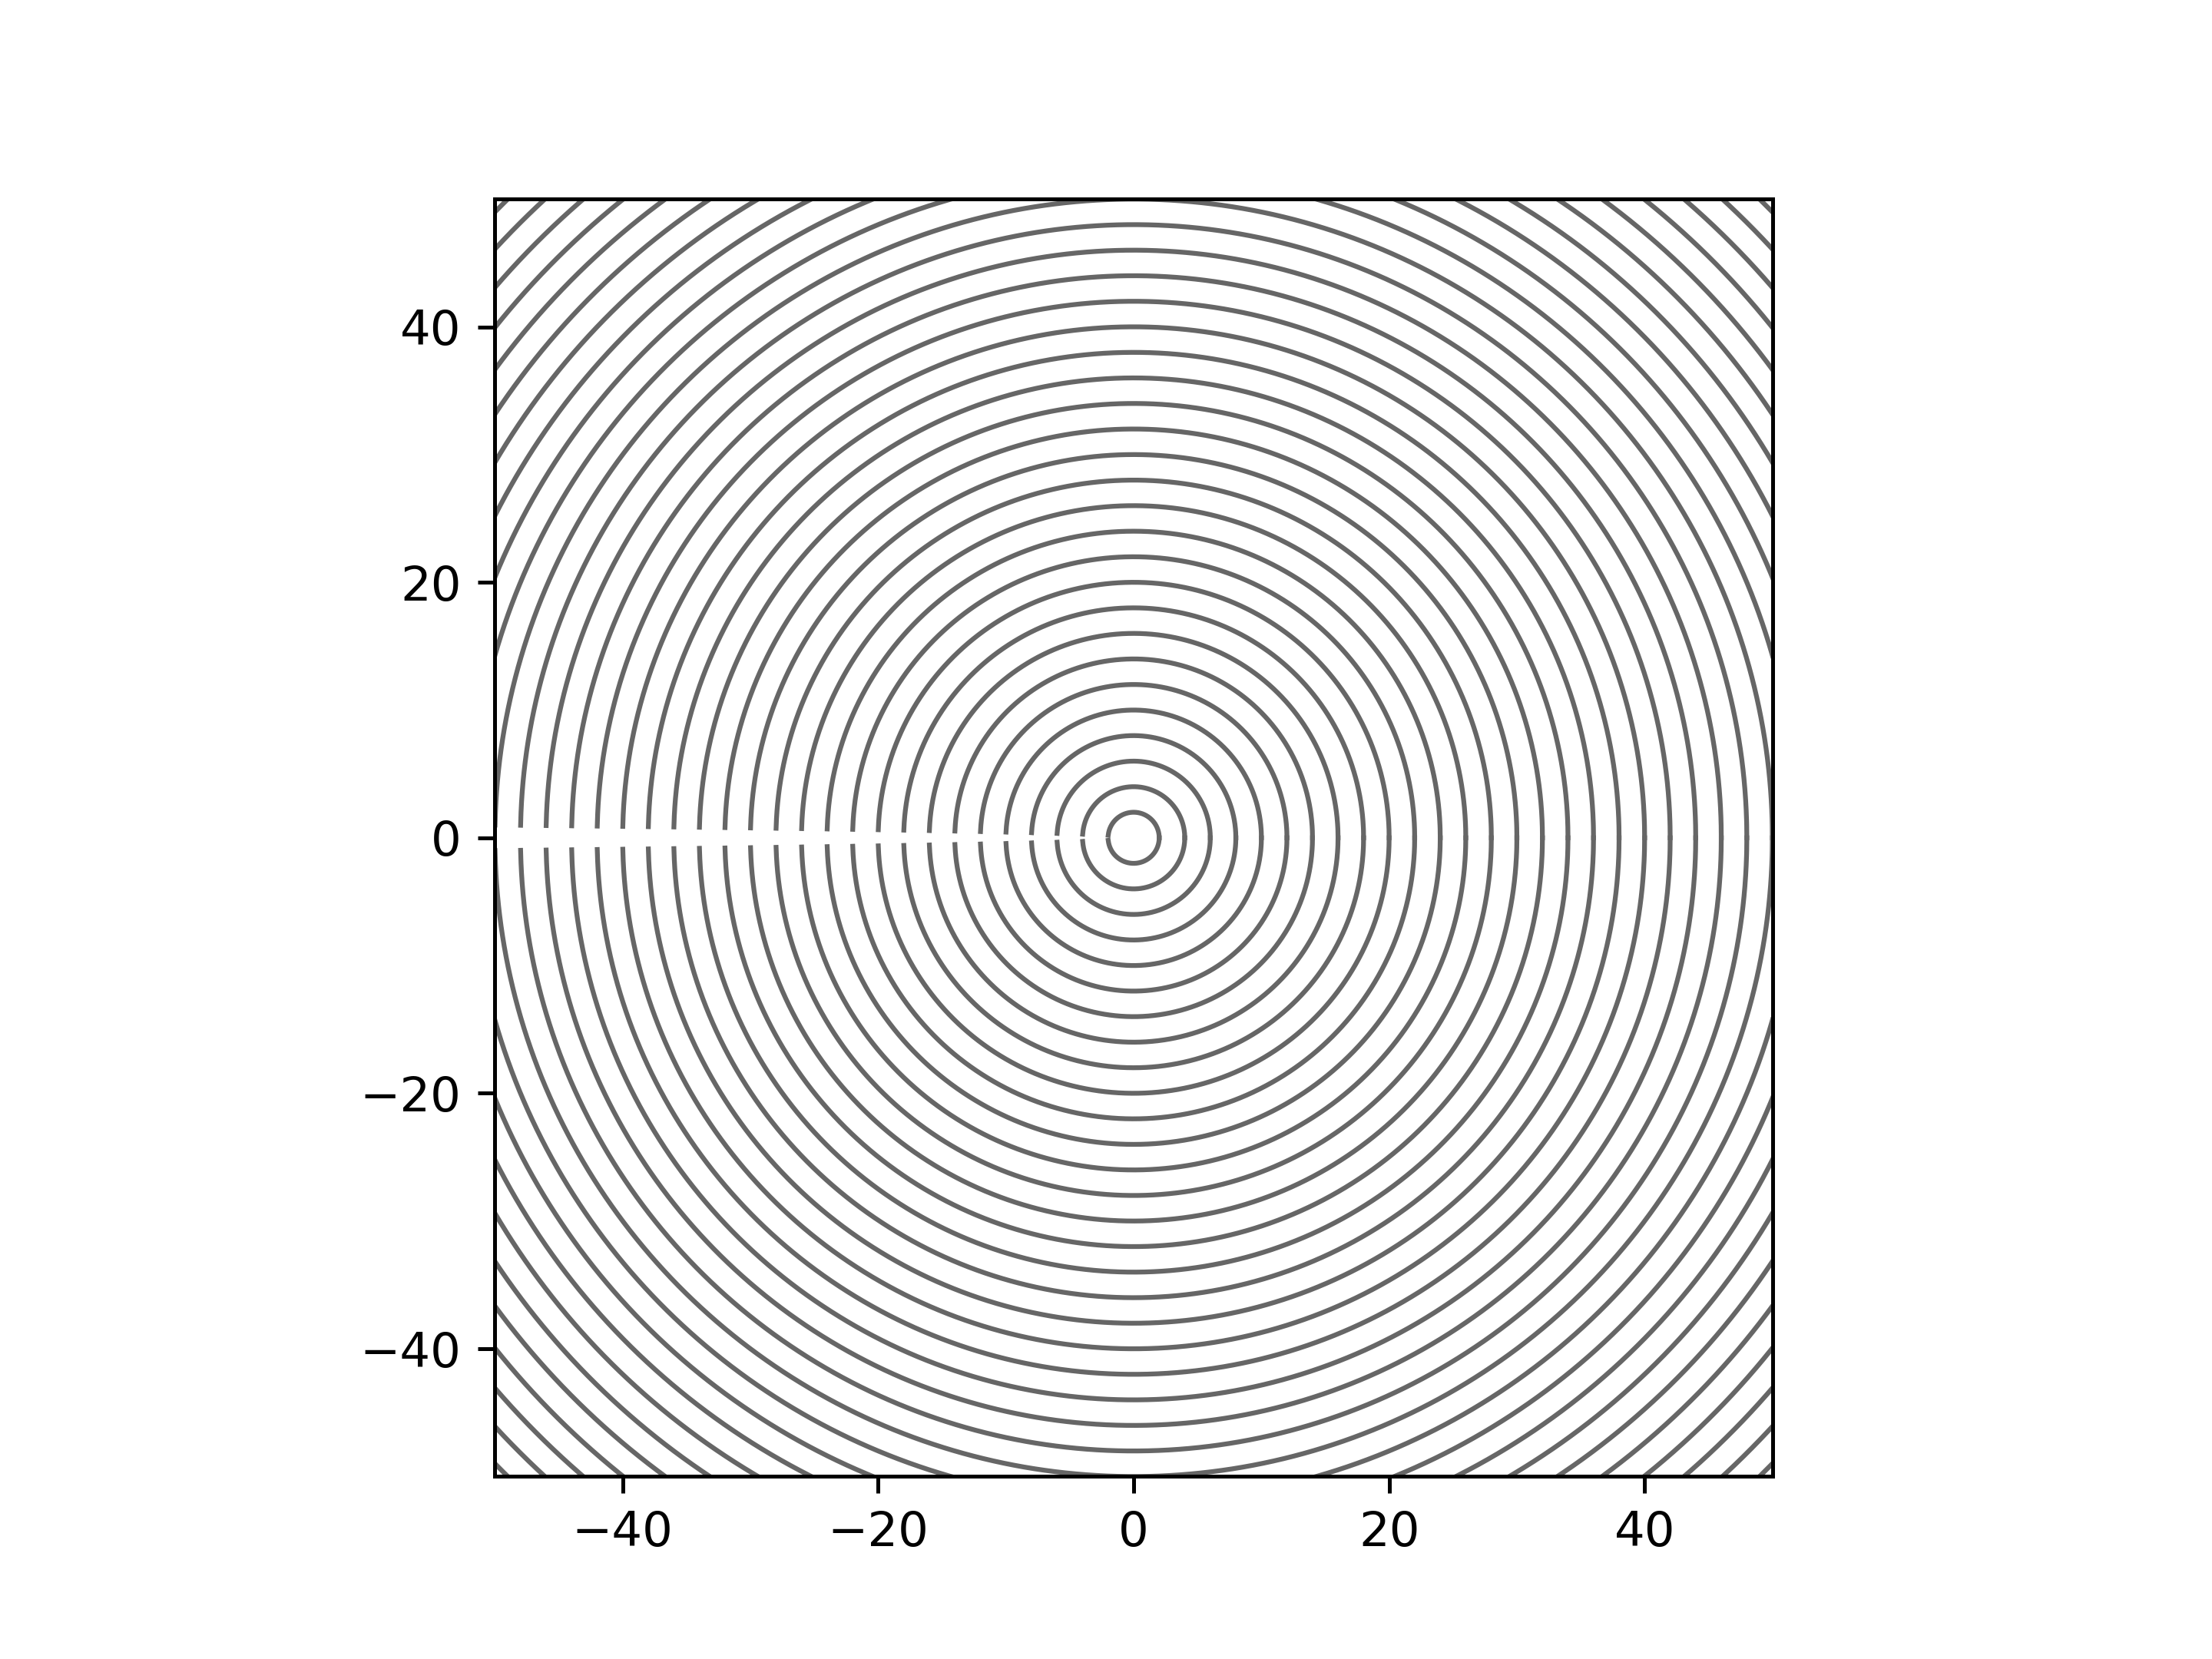
\includegraphics[height = 0.8\textheight]{assets/circle.png}
    \caption{Plot of possible circular orbits with the origin as the center.}
    \label{fig:my_label}
\end{figure}

\end{frame}

\subsection{Elliptical orbits}
\begin{frame}{\subsecname}

We obtain this orbit when \(\varepsilon \in (0,1)\) which gives us

\begin{equation}
    r = \frac{r_0}{1- \varepsilon \cos \theta} > 0
\end{equation}

for all \(\theta\). This means that \(r\) remains finite since the denominator will never be 0.

\end{frame}

\begin{frame}{\subsecname}
\begin{figure}
    \centering
    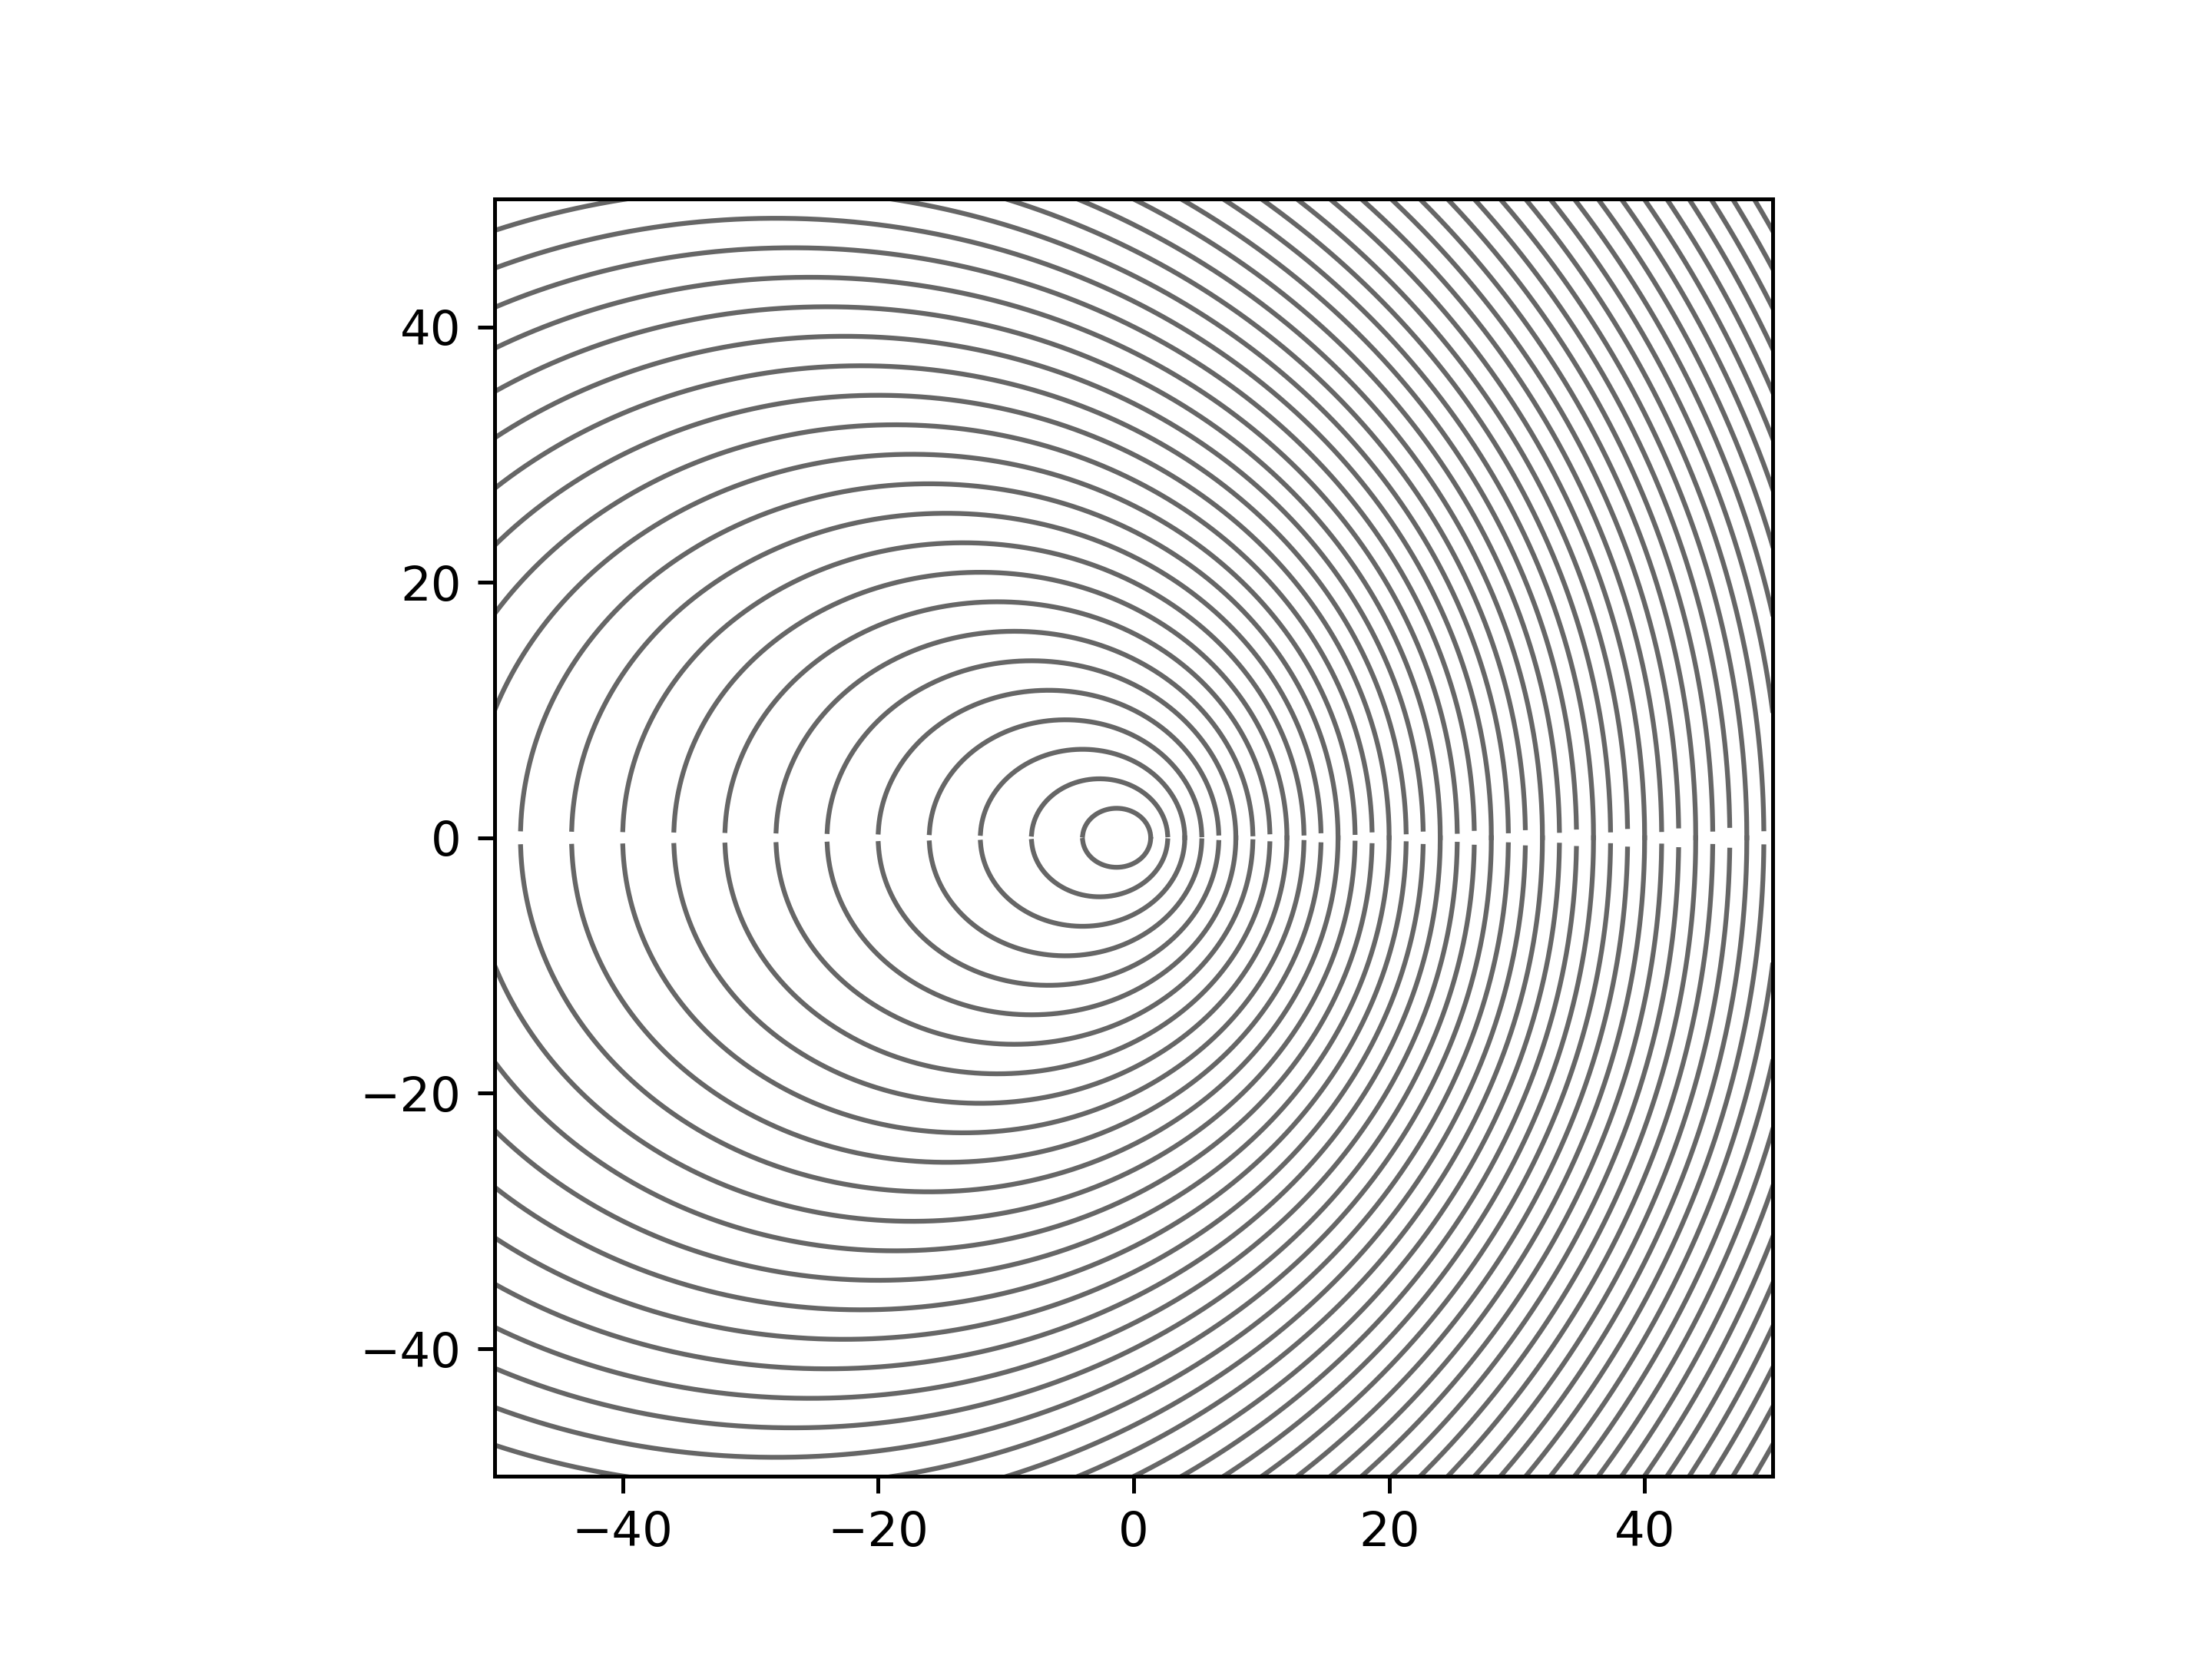
\includegraphics[height = 0.8\textheight]{assets/ellipse.png}
    \caption{Plot of possible elliptical orbits. Note that the origin is one of the foci.}
    \label{fig:my_label}
\end{figure}
\end{frame}

\subsection{Parabolic orbits}
\begin{frame}{\subsecname}

We obtain this orbit when \(\varepsilon = 1\) which gives us

\begin{equation}
    r = \frac{r_0}{1-\cos \theta}.
\end{equation}

Note that as \(\theta \to \pi/2 \), \(1-\cos \theta \to 0\), and it follows that \(r = \frac{r_0}{1-\cos\theta} \to \infty\). This is the first case where the body reaches escape velocity. 

\end{frame}

\begin{frame}{\subsecname}
\begin{figure}
    \centering
    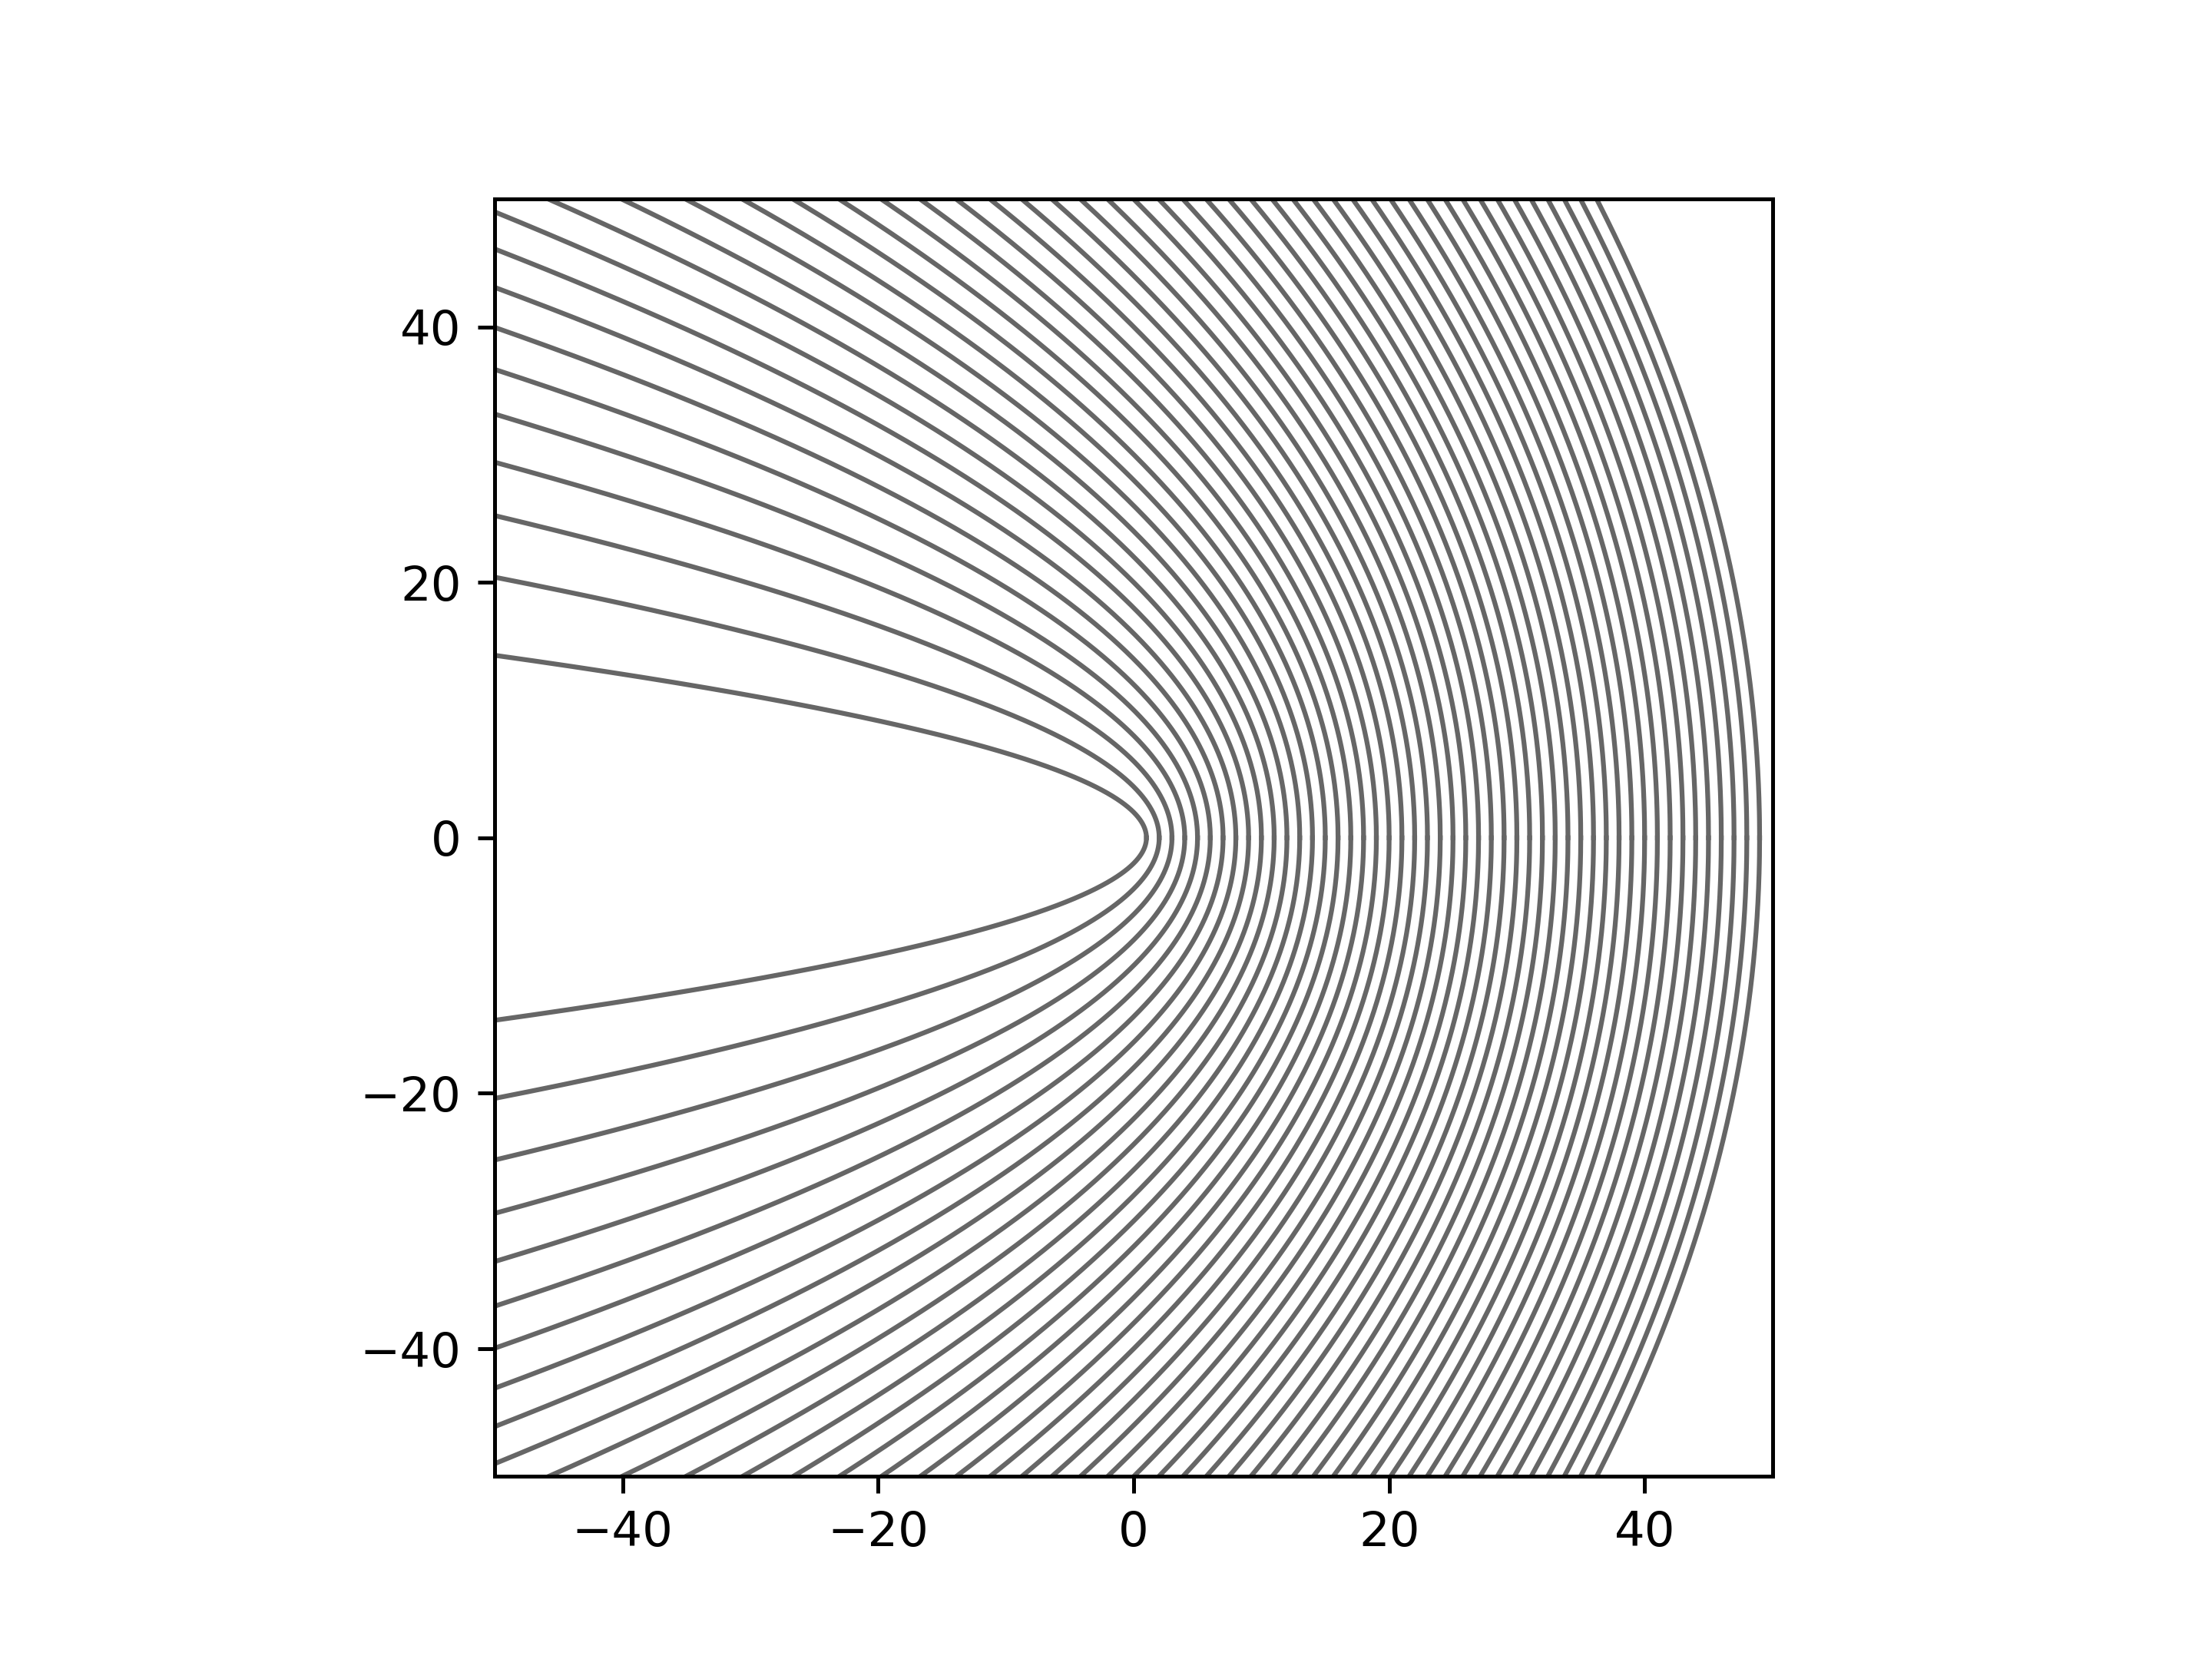
\includegraphics[height = 0.8\textheight]{assets/parabola.png}
    \caption{Plot of possible elliptical orbits. Note that the origin is the focus.}
    \label{fig:my_label}
\end{figure}
\end{frame}

\subsection{Hyperbolic orbits}
\begin{frame}{\subsecname}

We obtain this orbit when \(\varepsilon > 1\) which gives us

\begin{equation}
    r = \frac{r_0}{1- \varepsilon \cos \theta}
\end{equation}

which can go negative.

\end{frame}

\begin{frame}{\subsecname}
\begin{figure}
    \centering
    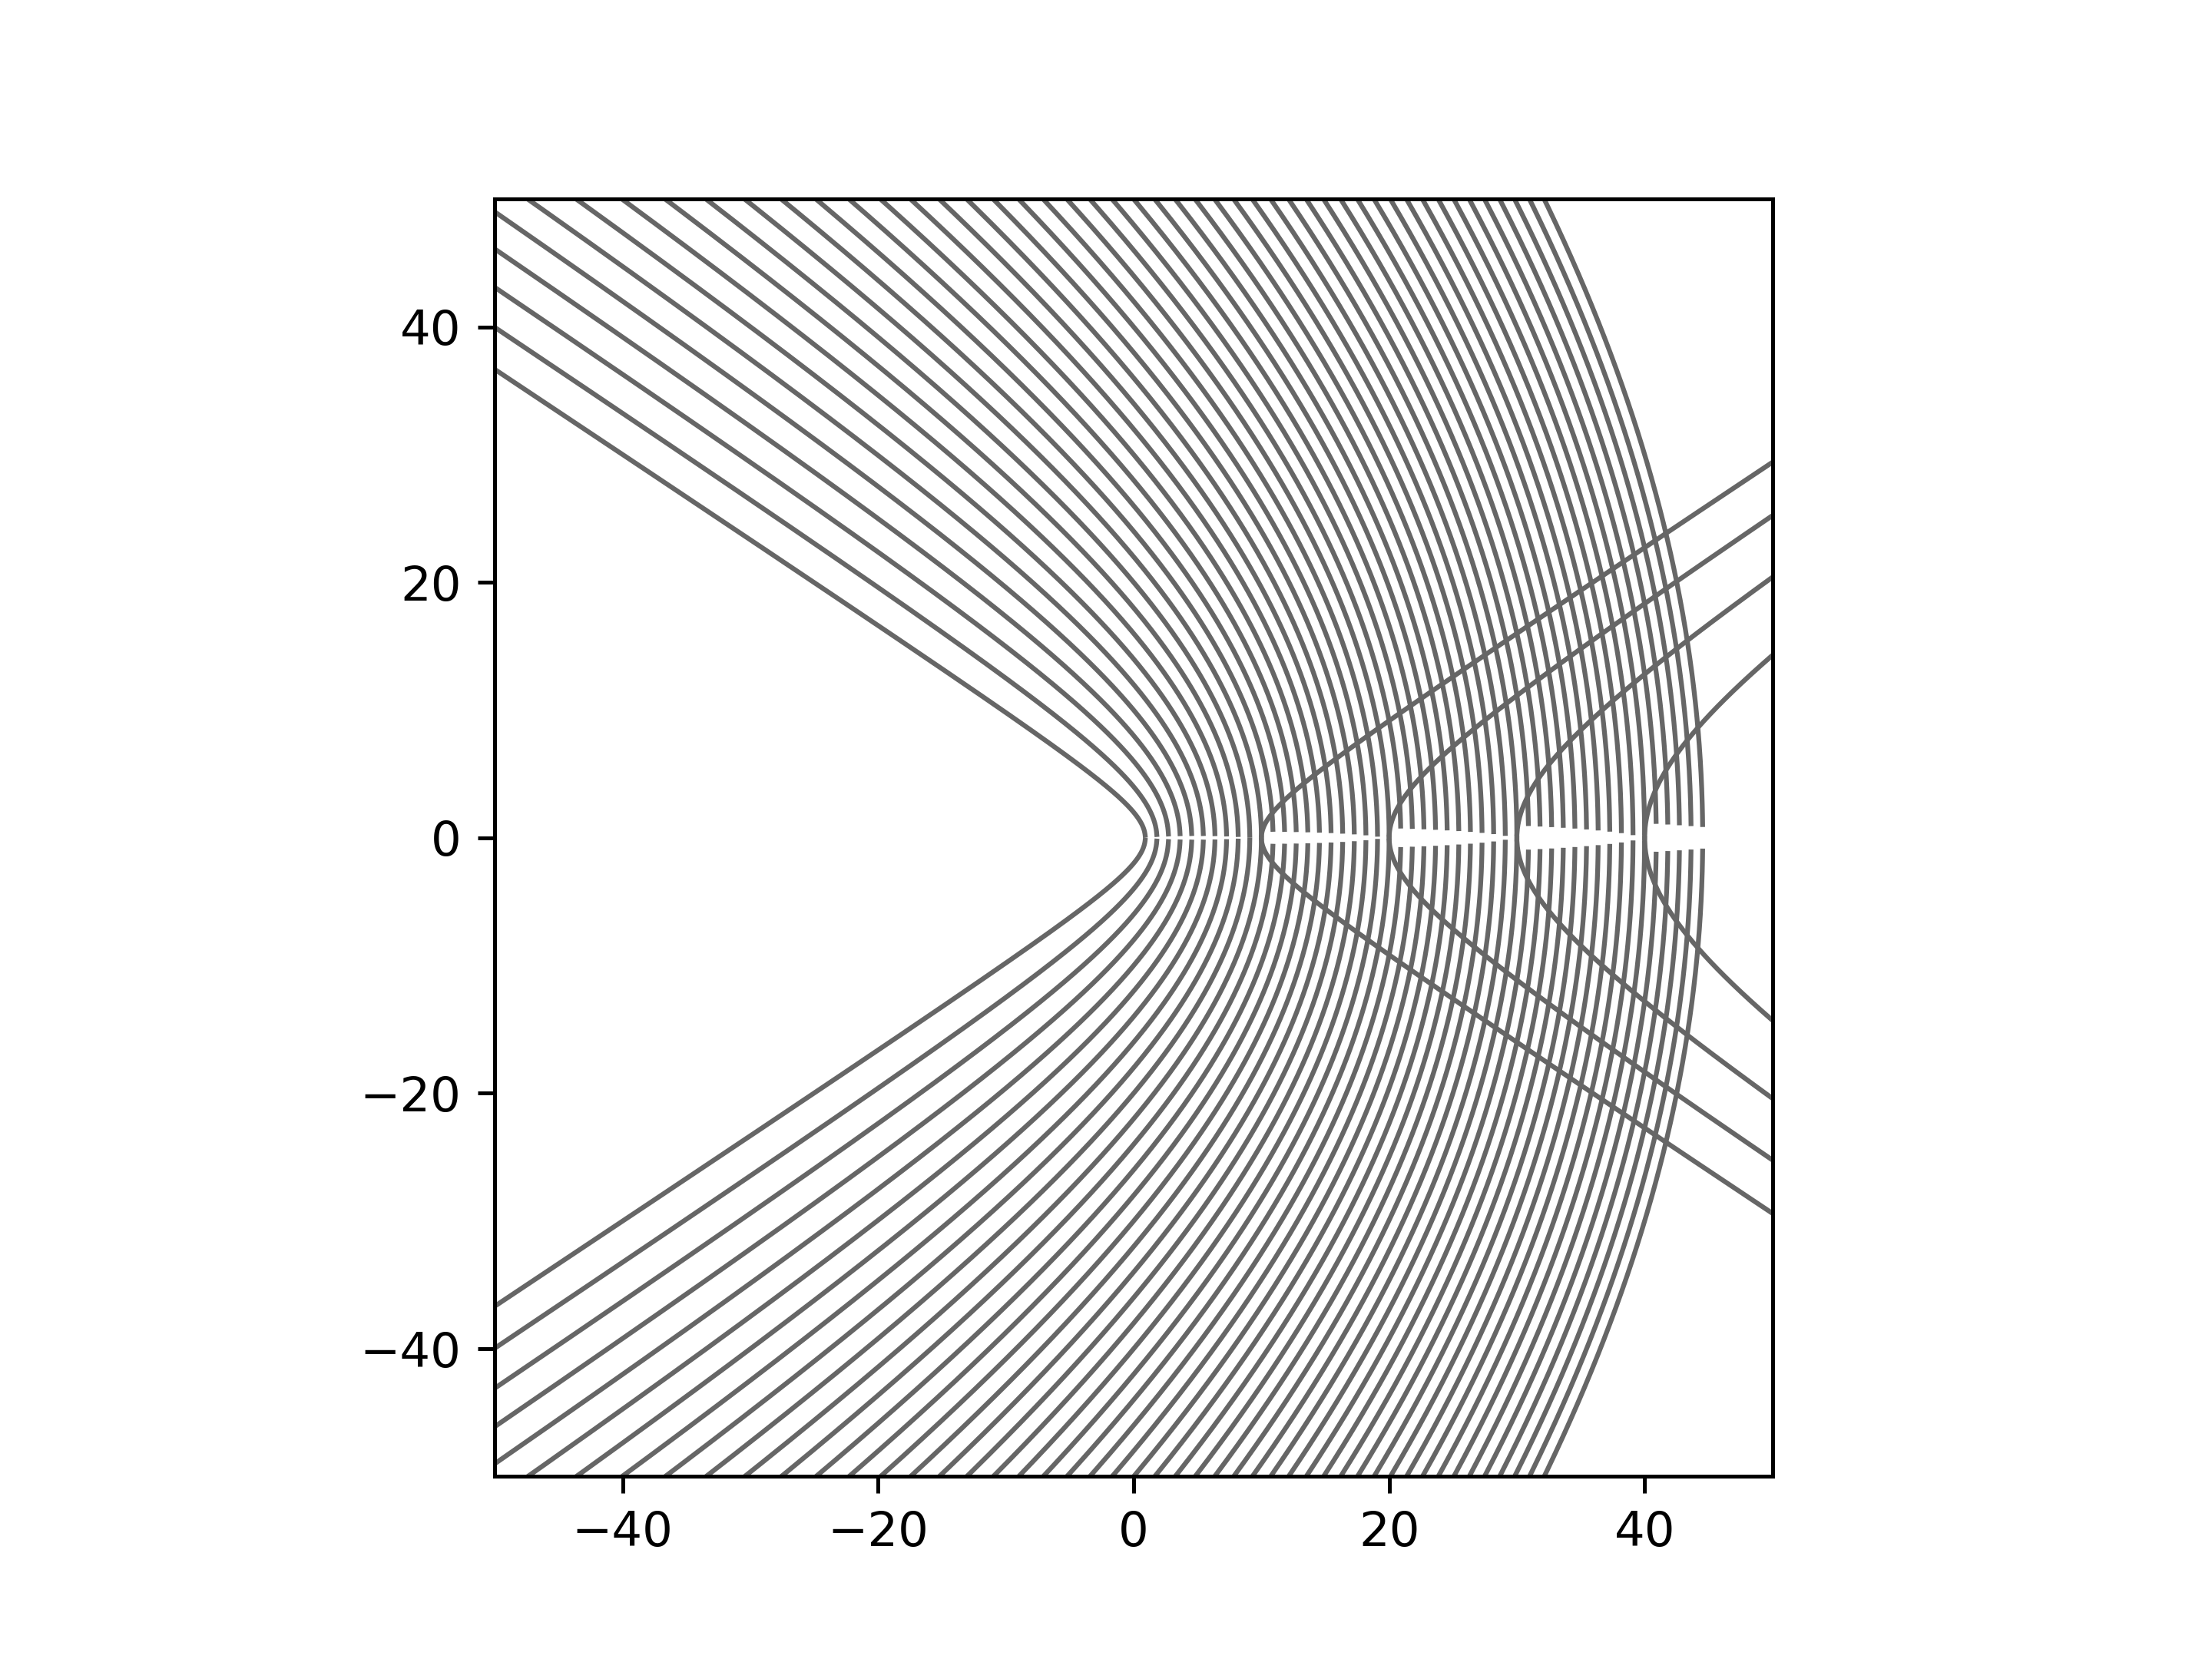
\includegraphics[height = 0.8\textheight]{assets/hyperbola.png}
    \caption{Plot of possible hyperbolic orbits.}
    \label{fig:my_label}
\end{figure}
\end{frame}

\section{Applications}
\subsection{Escape velocity}

\begin{frame}{\subsecname}

Note that orbits that escape the gravitational pull of a body has \(\varepsilon > 1\). From Equation \ref{tot_e}, 

\begin{equation}
E = \frac{Gm_1m_2(\varepsilon^2-1)}{2r_0} = \frac{1}{2} \mu v^2 - \frac{Gm_1m_2}{r}
\end{equation}

Hence we can isolate \(v\) and obtain

\begin{equation}
v = \left[\frac{Gm_1m_2(\varepsilon^2-1)}{\mu r_0} + \frac{2Gm_1m_2}{\mu r}\right]^{\frac{1}{2}} \geq  \left(\frac{2Gm_1m_2}{\mu r}\right)^{\frac{1}{2}}
\end{equation}

\end{frame}

\begin{frame}{\subsecname}

\begin{block}{Escape velocity}
In order for two objects to escape their gravitational interaction, their relative speed should be \(v\) such that

\begin{equation}
v \geq \left(\frac{2Gm_1m_2}{\mu r}\right)^{\frac{1}{2}}
\end{equation}

where \(\frac{1}{\mu} = \frac{1}{m_1} + \frac{1}{m_2}\).

\end{block}

\end{frame}

\begin{frame}{Special case}

Suppose the system consists of a small body and a big body. Without loss of generality, let \(m_2\) be the mass of the large object. Hence

\begin{equation}
\frac{1}{\mu} = \frac{1}{m_1} + \frac{1}{m_2} \approx \frac{1}{m_1} \implies \mu = m_1
\end{equation}

\end{frame}

\begin{frame}{Special case}

\begin{block}{Escape velocity from a large body}
In order for a small body to escape the gravitational influence of a larger body, the smaller body should be travelling at a velocity \(v_\text{small}\) such that 

\begin{equation}
v_\text{small} \geq \left(\frac{2Gm_2}{r}\right)^{\frac{1}{2}}
\end{equation}

where \(m_2\) is the mass of the larger body.

\end{block}

\end{frame}


\begin{frame}{Solving for Earth's escape velocity}
Given \(m_2 = 5.972 \times 10^{24} \text{kg}\) and \(r = 6.3781 \times 10^6 \text{m}\) and letting \(m_1 = 1000.0 \text{kg}\),

\begin{align}
v \approx 11180 \text{m} \cdot \text{s}^{-1} && v_\text{small} \approx 11180 \text{m} \cdot \text{s}^{-1}
\end{align}
\end{frame}

\subsection{Geostationary orbit}

\begin{frame}{\subsecname}
A geostationary orbit is a circular geosynchronous orbit on Earth with an orbital period equal to Earth's rotational period.

Given \(\varepsilon = 0\),

\begin{equation}
E = -\frac{Gm_1m_2}{2r} = \frac{1}{2} \mu v^2 - \frac{Gm_1m_2}{r}
\end{equation}

\begin{block}{General and special models for geostationary orbits}
\begin{equation}
v = \left(\frac{Gm_1m_2}{\mu r} \right)^\frac{1}{2} \approx  \left(\frac{Gm_2}{r} \right)^\frac{1}{2}
\end{equation}
\end{block}
\end{frame}

\begin{frame}{Solving for the geostationary orbit altitude}
Let \(v = \frac{2\pi r}{T}\) where \(T\) is the orbital period and \(r\) is the radius of the orbit.

Given \(T = 86164 \text{s}\), \(m_1 = 1000.0 \text{kg}\), and \(m_2 =  5.972 \times 10^{24} \text{kg}\),

\begin{equation}
r = \left(\frac{Gm_1m_2T^2}{4\mu\pi^2}\right)^{\frac{1}{3}} \approx 4.216 \times 10^{7} \text{m} \approx 42160 \text{km}.
\end{equation}

Given \(r_\text{earth} = 6.3781 \times 10^{6} \text{m}\), the altitude of the body -- we denote by \(h\) -- is 

\begin{equation}
h \approx 4.216 \times 10^{7}m  - 6.3781 \times 10^{6} \text{m} \approx 35790 \text{km}.
\end{equation}

\end{frame}

\maketitle

\end{document}